\section{HMM}\label{hmm}
teoria del TTS donde entra el cuadro general con vocoder y explicar glott y straight un poco (no se si aqui o en subseccion aparte)
The Hidden Markov Model (HMM) is one the statistical time series model most used in different fields. It has been used in speech recognition for years with great success and also TTS systems has made substantial progress in the last years using HMM.\\
A HMM is a finite state machine which generates a sequence of discrete time observations. At each time unit, the HMM change the state at Markov process with a state transition probability and the generates observational data in accordance with an output probability distribution of the current state.\\
A N-state HMM machine is defined by the state transition probability (A), the output probability distribution (B) and initial state probability ($\Pi$). Typical HMM structures can be seen in figure \ref{hmmstruct}.\\
\begin{figure}[!htb]
	\begin{center}
	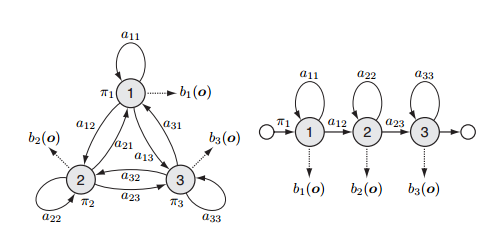
\includegraphics[width=1\textwidth]{img/hmmstruct.png}
	\end{center}
	\caption{\label{hmmstruct}Typical HMM structures \ref{junichi hts intro}}
\end{figure}
The structure on the left of figure \ref{hmmstruct} is a 3-state ergodic model, in which all states can be reached by the others in a single transition. The structure on the right is a 3-state left to right model, in which the state index simply increases or stays depending on the time increment. This last model is often used as speech units to model speech parameter sequences since they can appropriately model signals whose properties successfully change.\\
\clearpage%%si no funciona poner newpage pero me hacia cosas raras con las imagenes
\section{HMM-Based Speech Synthesis}\label{hmmbased}
Here an HMM-based text-to-speech system is described. In the HMM-based speech synthesis, the speech parameters of a speech unit are statistically modeled and generated using HMMs based on maximum likelihood criterion \ref{una de las de junichi}.\\

Explicar como funciona un poco ain meternos en el modelo matematico parametros training etc

Luego decir que el HTS puede usar varios vocoder para sintetizar y analizar y hablar ahi de straight (mepcepstral etc) y de glott.
 A lo mejor buena idea hablar de straight y glott en el analisis para diferenciar un poco training comun y luego volver a hablar de cada uno en synthesis
 Mejor un poco en general del HMM con training y sinthesis como tiene tuomo y luego explico un poco mas personalizado analsis y synthesis para straight y glott como tiene manu\\
 
The main goal of the TTS system is to produce natural synthetic speech sound including different types of speaking and emotions. In order to achieve this the system can be divided into two main parts: training and synthesis, as it is illustrated in figure \ref{ttsstruct}. The analysis is considered as part of the training and is where the features are extracted from the speech database. This features are then modeled by HMM. In the synthesis part, the HMMs are concatenated according to the analyzed input text and speech parameters are generated from the HMM, then the synthesis module transforms them into a speech waveform.\\
\begin{figure}[!htb]
	\begin{center}
	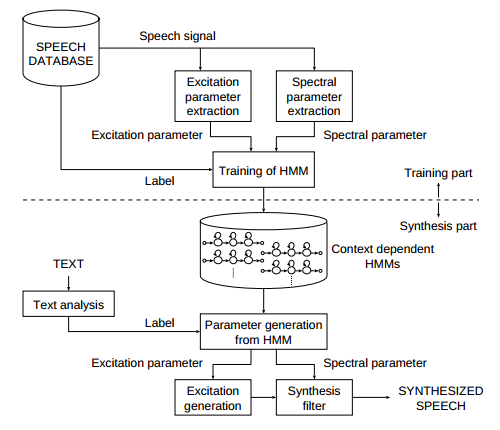
\includegraphics[width=1\textwidth]{img/ttsstruct.png}
	\end{center}
	\caption{\label{ttsstruct}TTS overview \ref{articulo an hmm-based...}}
\end{figure}
\subsection{Training Part}\label{tpart} 
As it has been seen (section \ref{hmmbased}) this training part is divided into two stages: the parametrization or feature extraction and the HMM training.\\
In the parametrization stage the input speech signal is compressed into a few parameters which would describe its characteristics as accurately as possible. This stage is done in a different ways depending on the vocoder that is being used and will be explained in section \ref{voco-a-s} and for more detail see \ref{tuomo} \ref{manu}.\\
In the HMM training stage the features obtained are modeled simultaneously by HMM. First monophone HMM models are trained in a 7-state left-to-right structure with 5 emitting states. All the parameters excluding the F0 are modeled with continuous density HMMs by single Gaussian distributions with diagonal covariance matrix. F0 is modeled with by a multi-space probability distribution (MSD-HMM) \cite{introhmmbased} due to the conventional continuous or discrete HMMs models can not be applied to F0 pattern modeling because F0 is composed of one-dimension continuous values and a discrete symbol that represents the unvoice. The state duration for each HMM are modeled with multidimensional Gaussian distributions. For GlotHMM (Y NO SE PARA STRAIGHT!!!) each feature is modeled in an individual stream  and for the F0 due to the MSD-HMM three streams are used, so the model has eight streams. In order to smooth transitions between states in parameter generation the delta and delta-delta coefficients of each feature are calculated, so the total feature order is 171.\\
After the training of the monophone HMMs the monophone models are converted into context dependent models. As the number of contextual factor increase, their combination increase exponentially. So with limited training data models parameters can not be accurately estimated and it is impossible to prepare a speech database that covers all combinations of contextual factors. To overcome this problem, the models for each feature are clustered independently by using a decision-tree based context clustering (Figure \ref{decision-tree}). In order to generate synthesis parameters for new observations vectors that are not included in the training data the clustering is also required.
\begin{figure}[!htb]
	\begin{center}
	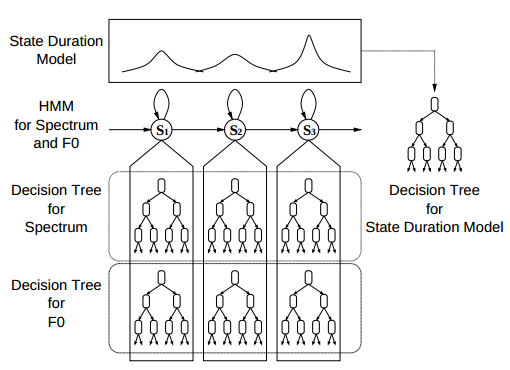
\includegraphics[width=1\textwidth]{img/decision-tree.png}
	\end{center}
	\caption{\label{decision-tree}Example of decision-tree based context clustering for some features \ref{articulo an hmm-based...}}
\end{figure}
\subsection{Synthesis Part}\label{synpart}
In this part the model created in the training part is used to generate speech parameters according to a text input. With this parameters the synthesis module is able to generate a speech waveform. So the synthesis part has two stages: the parameter generation and the synthesis as is illustrated in figure \ref{syngen}.\\
In the parameter generation stage, the text input is first  converted into to a context based label sequence by performing  phonological and high level linguistic. According to the decision trees generated in the training stage and the label sequence, a sentence HMM is generated by concatenating the context dependent HMMs. The state durations of the sentence HMM  are determined so as to maximize the likelihood of the state duration densities. With the sentence and the state durations, a sequence of speech features are generated and then used by the synthesis module to generate the speech waveform.\\
\begin{figure}[!htb]
	\begin{center}
	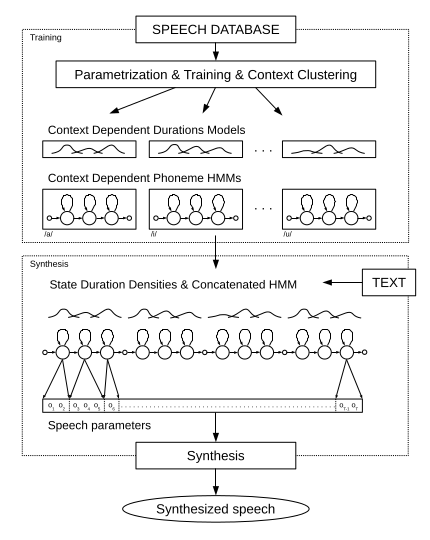
\includegraphics[width=0.9\textwidth]{img/syngen.png}
	\end{center}
	\caption{\label{syngen}HMM-based generation process of speech parameters \ref{Tuomo}}
\end{figure}
In the synthesis stage, as it has already been said, the speech waveform is generated according to the features generated in the first stage of the synthesis part. This synthesis stage differs depending of the vocoder used, so it will be explained in section \ref{voco-a-s}.
\clearpage
\section{Vocoders}\label{voco-a-s}
Many different vocoders has been developed to be applied with HMM-based speech synthesis (see \ref{manu thesis}). In this section two of them will be explained: GlotHMM and Straight due to they are the ones that are being compared in this project.
\subsection{GlotHMM}\label{glotthmmvoco}
The GlotHMM was proposed by Tuomo Raitio \cite{tuomo}. GlotHMM estimates the real glottal pulse signal G(z) an the vocal tract filter V(z) associated with it. So the speech signal can be represented as:
\begin{equation}
	S(z) = G(z)V(z)L(z) 
\end{equation}
where L(z) represents the lip radiation. All parts are estimated of real physical properties. For example the glottal pulse signal can be divided into the source part E(z) an the filter containing the spectral envelope of the glottal pulse F$_{G}$(z):
\begin{equation}
	G(z) = F_{G}(z)E(z)
\end{equation}
and so the vocal tract filter can be expressed as:
\begin{equation}
	V(z) = \dfrac{F(z)}{F_{G}(z)L(z)} 
\end{equation} %%peta y no se xq si lo pongo bien con graccion
To extract the parameters (analysis) of the speech signal GlottHMM follows this steps:
\begin{itemize}
	\item First, the speech signal is high-pass filtered and windowed into fixed length rectangular frames, from which the signal log energy is calculated as a feature parameter
	\item Second, the Iterative Adaptive Inverse Filtering (IAIF) algorithm illustrated in figure \ref{iaif} and explained in \ref{manu}, is applied to each frame and results in the LPC representation of the vocal tract spectrum and and the waveform representation of the voice source
	\item The LPC spectral envelope estimate of the voice source is calculated , and along with the LPC estimate of the vocal tract spectral envelope, is converted into LSF representation
	\item The glottal flow waveform is used also for the acquisition of the F0 value as well as the Harmonic-to-Noise Ratio (HNR) values for a predetermined amount of sub-bands frequency. 
\end{itemize}
\begin{figure}[!htb]
	\begin{center}
	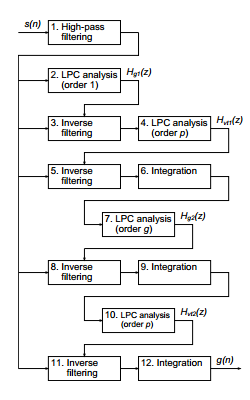
\includegraphics[width=0.7\textwidth]{img/iaif.png}
	\end{center}
	\caption{\label{iaif}IAIF algorithm block diagram \ref{Tuomo}}
\end{figure}
The output of the IAIF algorithm g(n) (estimated glottal flow signal) is used to generate the rest of the analysis parameters. A voicing decision is made based on the amount of zero-crossing and low-band energy. For voiced frames, the F0 value of the frame is estimated using the autocorrelation method. The HNR is calculated from g(n). For unvoiced frames the HNR and F0 are set to zero. The F0, HNR and the source LSF are used to model the excitation signal that is filtered by the vocal tract filter.\\
The final analysis vector of GlotHMM consists of single parameters for the F0 and log energy, around 5 parameters for HNR, 10-20 parameters for the glottal source LSF parameters and 20-30 parameters for the vocal tract LSF parameters.\\ 
To perform the synthesis GlottHMM uses a method for the excitation generation based on the voice/unvoice decision instead of using a traditional mixed excitation model. The synthesis block diagram is illustrated  in figure \ref{gsynb}.\\
\begin{figure}[!htb]
	\begin{center}
	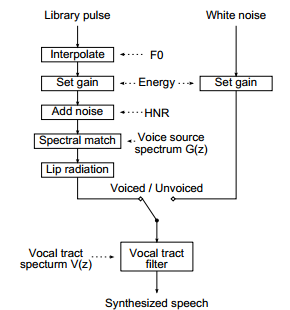
\includegraphics[width=0.7\textwidth]{img/gsynb.png}
	\end{center}
	\caption{\label{gsynb}Synthesis block diagram for GlotHMM vocoder \ref{Tuomo}}
\end{figure}
For the voiced frames, the heart of the synthesis procedure is a fixed library pulse that is obtained by glottal inverse filtering a sustained vowel signal. The library pulse is interpolated to match the target F0 value using cubic spline interpolation, and its energy is set to match the target gain obtained from the analysis vector.\\
Next, a HNR analysis is done to the library pulse. For each sub-band, noise is added to the real an imaginary parts of the FFT vector according to the differences between the obtained and the target HNR values.\\
The spectrum of the library pulse is matched to the spectrum of the target glottal pulse obtained from the analysis vector. The spectral matching is done by performing LPC analysis to the library pulse, and then filtering the obtained residual with the target synthesis filter. Finally, the lip radiation effect is added to the excitation by filtering it with a fixed differentiator.\\
For unvoiced frames, the excitation is generated as white Gaussian noise whose gain is set by the energy parameter of the analysis vector.\\
The excitation is combined in the time domain by overlap-adding target frames, and the final synthetic signal is generated by filtering the excitation with the vocal tract filter derived from the vocal tract LSFs obtained from the analysis vector.\\
\subsection{STRAIGHT}\label{straightvoco}
STRAIGHT (Speech Transformation and Representation using Adaptive Interpolation of weiGHT spectrum) is the more established of the more sophisticated vocoding methods. Proposed by Kawahara in 1977, it has gone through extensive research and development since then. Is often the main reference to which other vocoders in HMM-based synthesis are compared, like in the case of this project.\\
For HMM synthesis some modifications were made and now the spectral envelope is represented as mel-frequency cepstral coefficients, and the corresponding aperiodicity measurements are averaged over five sub-bands frequency.\\
In the parameter extraction (analysis) the main idea behind STRAIGHT is the extraction of a smoothed spectral envelope , which minimized the effect of periodicity interference in the analysis frames. This means that the spectral envelope is essentially independent of the speech excitation, which is a great feature with respect to speech transformation.\\
The extraction of the spectral envelope can be found in \ref{manu}.\\
The spectrum is represented as mel-frequency cepstral representation for the purpose of statistical modeling. The aperiodicity measurements are also transformed into a compressed representation. \\
The acquired analysis vector for STRAIGHT consists of the F0 value, five aperiodicity coefficients and 20-40 spectral MFC coefficients (MFCCs). \\
STRAIGHT synthesis is done in frame-by-frame basis by creating a mixed excitation signal of the length of two pulse periods based on the F0 and aperiodicity measurements. The harmonic pulse train is all-pass filtered with a randomized group-delay filter, which reduces the buzziness of the resultant synthesis. The acquired mixed excitation signal is convolved with the minimum phase MLSA filter derived from the frame's spectral MFCCs. Finally, the Pitch-Synchronous Overlap-Add (PSOLA) algorithm is applied to the synthesized frames to get the speech waveform signal.  
\begin{figure}[!htb]
	\begin{center}
	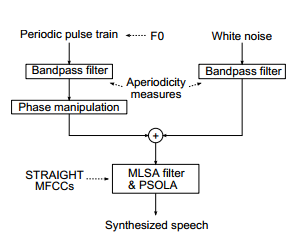
\includegraphics[width=0.7\textwidth]{img/ssynb.png}
	\end{center}
	\caption{\label{ssynb}Synthesis block diagram for STRAIGHT vocoder \ref{Tuomo}}
\end{figure}
As illustrated in figure \ref{ssynb} the components for the mixed excitation are generated by sub-band filtering the voice (impulse train) and unvoice (white Gaussian noise) parts separately in the frequency domain. The stepwise band-pass filters used are determined by the aperiodicity coefficients so that the resultant sub-bands will have the same average lower-to-upper envelope ratio as the respective aperiodicity coefficient.\\
After the sub-band weighting, the pulse train component is all-pass filtered to adjust the phase characteristics of the excitation.